\subsection{Aplicação Fábrica - Produção}
\subsubsection*{Descrição do caso de uso}
No registo de produção, espera-se que utilizador entre na página e indique o código de barras da recolha, o peso de cera, metal e plástico e o seu ID. A informação da data de produção deve ser indicada automaticamente pelo sistema e a informação sobre a recolha (ponto de recolha e data da recolha) seja obtido, em \textit{background}, após indicar o código de barras da recolha. A aparência da \textit{view} deste caso de utilização será semelhante ao demonstrado na figura \ref{fig:di_producao}.

\begin{figure}[H] 
	\begin{center}
		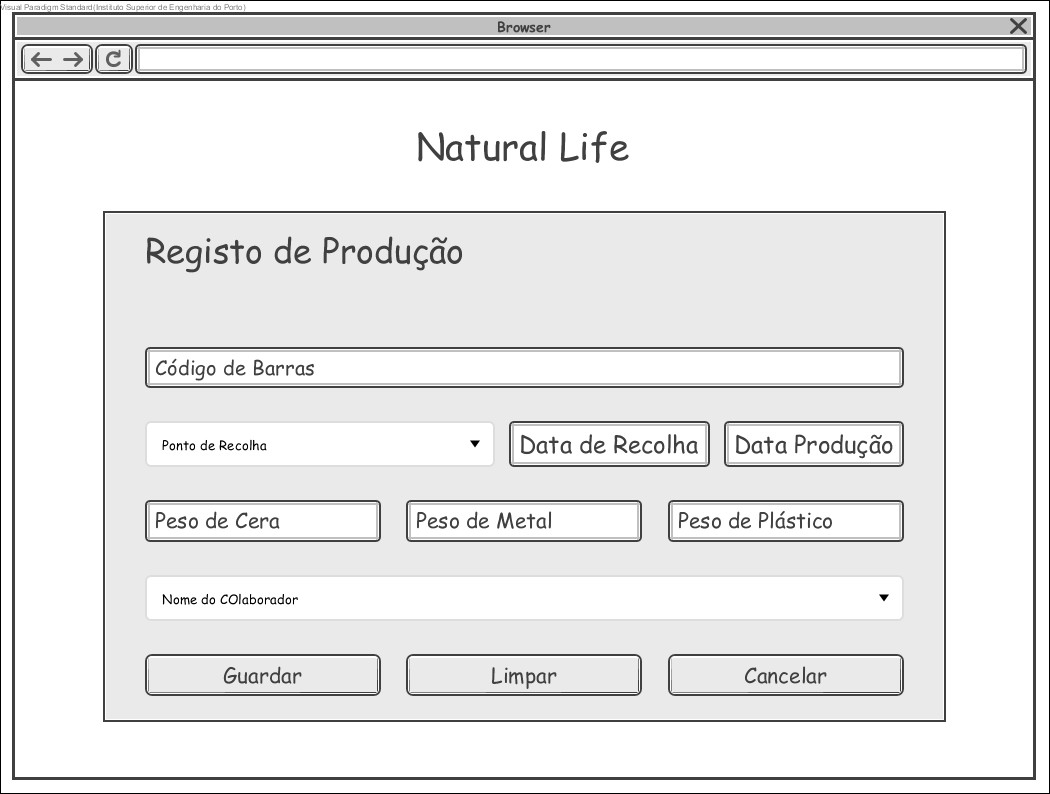
\includegraphics[width=0.57\textwidth,keepaspectratio]{figuras/Diagramas_vp/DI_Fabrica_3_Registo_de_Producao.jpg}
		\caption{Modelo do formulário do registo de produção}
		\label{fig:di_producao} 
	\end{center}
\end{figure}


\subsubsection*{Fluxo do caso de utilização}
O caso de uso inicia-se com a abertura da página do registo de produção. É apresentado o formulário com a data de produção previamente preenchida. O utilizador tem de indicar o código de barras da recolha, peso de cera, metal e plástico e o seu ID numa lista de \textit{dropdown}. Quando o utilizador termina de indicar o código da recolha é feito um \textit{request} ao servidor para saber o ponto de recolha e data da recolha. Essa informação é apresentada automaticamente ao utilizador Após indicar as informações solicitadas precisona o botão "Guardar". No final do registo é apresentada uma mensagem ao utilizador, tal como demonstrado na figura \ref{fig:sd_producao}.

\begin{figure}[h!] 
	\begin{center}
		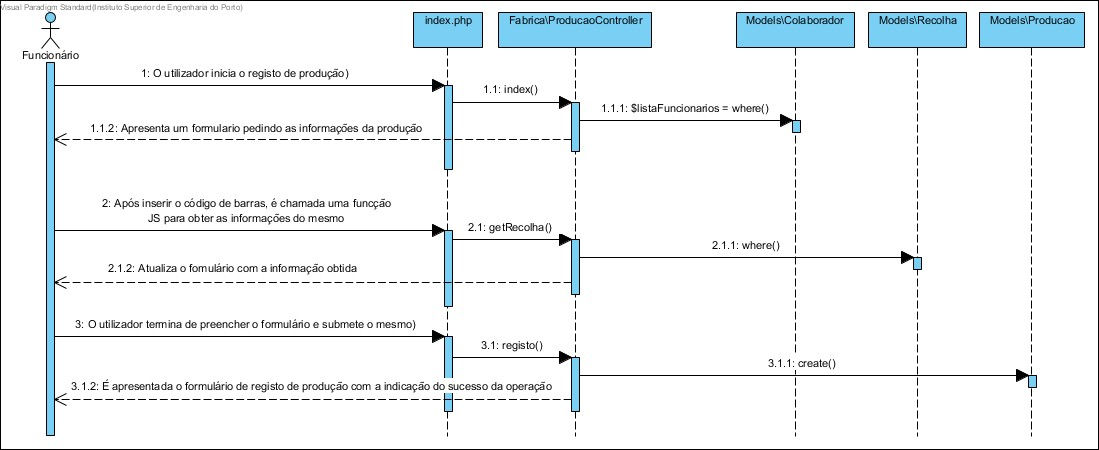
\includegraphics[width=0.93\textwidth,keepaspectratio]{figuras/Diagramas_vp/SD_Fabrica_3_Registo_de_Producao.jpg}
		\caption{Diagrama de sequência registo de produção}
		\label{fig:sd_producao} 
	\end{center}
\end{figure}
